\documentclass[heading.tex]{subfiles} 
\begin{document}

\section{Introduction}


The Hyperloop concept is a proposed transportation system aimed to lower costs and travel times relative to California's current high speed
 rail project. \cite{Musk} The design consists of a passenger pod traveling in a tube under light vacuum at ground level and near sonic
speeds. The capsule is supported by a set of air bearings with air provided by a battery powered compression system and propulsion maintained
by a set of linear actuators mounted to the tube. Even with the tube largely evacuated, the speed of the capsule is limited by the ability of air to
escape around the sides of the vehicle. This limitation is governed by the size of the capsule relative to the tube and is alleviated by redirecting air
through an inlet and compression system. Drawing sufficient airflow through the vehicle to support the bearings and achieve higher speeds results
in a fairly large air intake at the nose of the capsule, shown in Fig. \ref{f:hyperloopCAD}. The diameter of this inlet and hence the diameter of the
capsule, is strongly tied to the maximum travel speed of the capsule. This coupling between the maximum velocity and
required tube diameter cascades into multiple subsystems and needs to be accounted for upfront in the design process. 
All of the sub-system interactions make it necessary to take a more integrated approach to the design of the Hyperloop concept. The intention of
this paper is to explore some of the most significant trade-offs between sub-systems and provide a starting point for subsystem expansion.

\begin{figure}[hbtp]
\centering
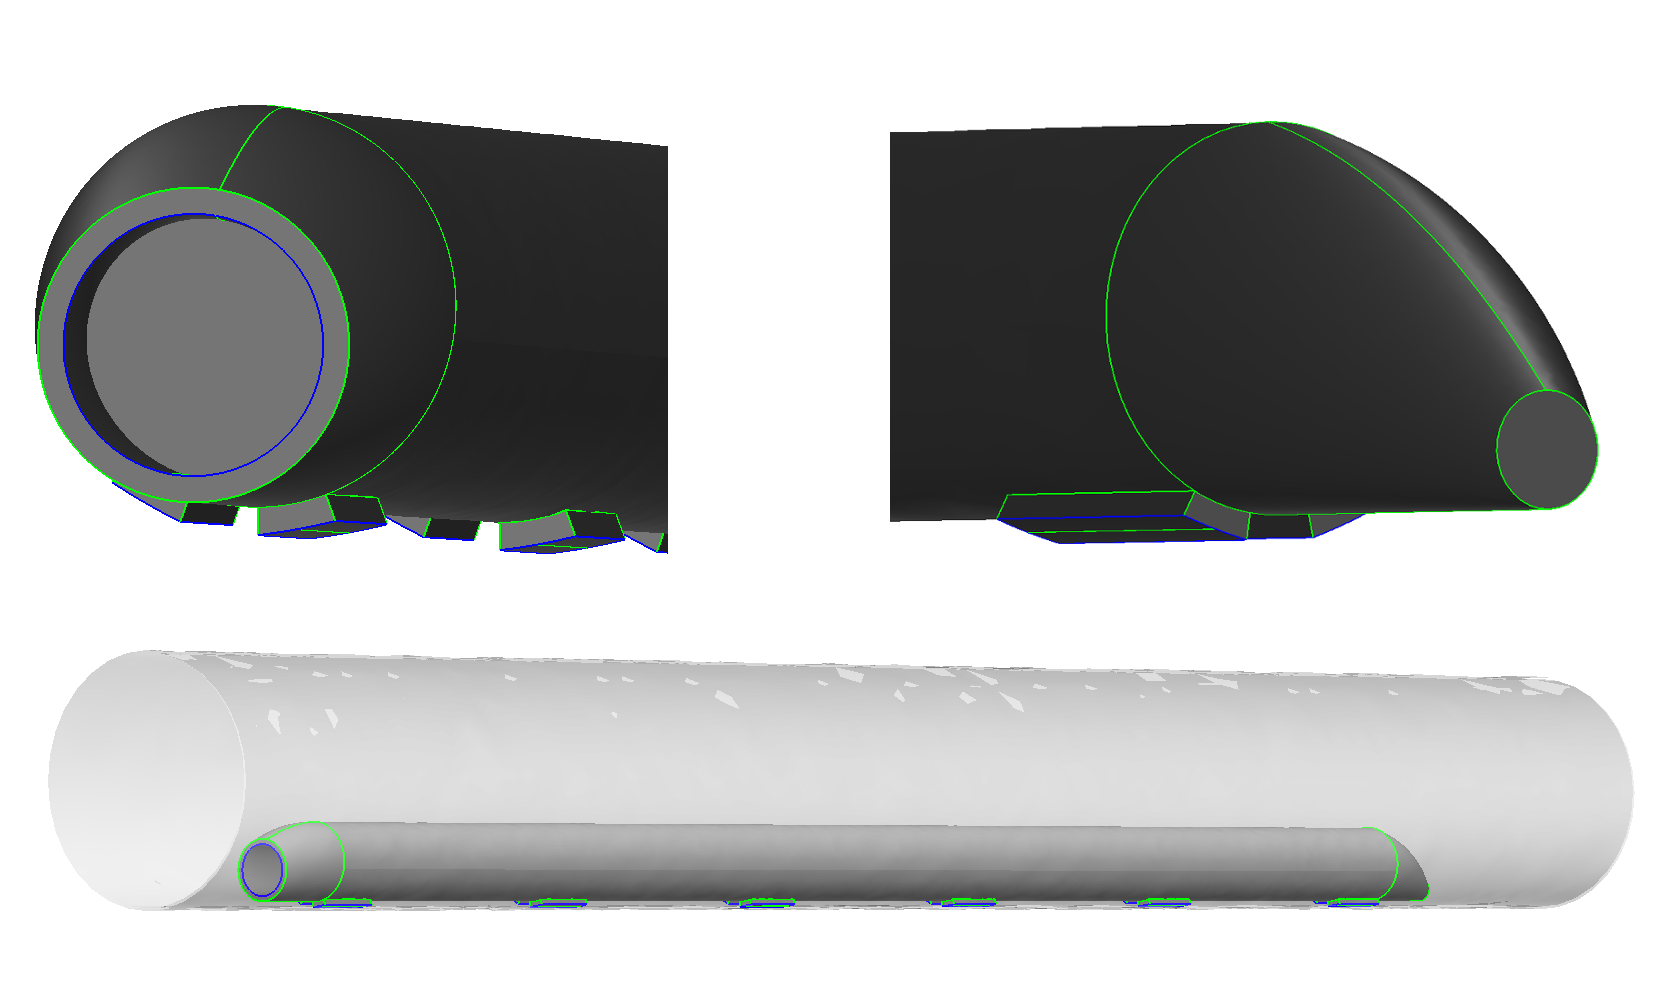
\includegraphics[width=\textwidth]{images/hyperloop_cad.png}
\caption{Calculated baseline inlet (left), nozzle (right), and full assembly (bottom) for a capsule speed of Mach 0.8, rendered in OpenCSM a parametric solid modeler.}
\label{f:hyperloopCAD}
\end{figure}

The physical limitations of the system and the underlying design space needs to be better understood before ultimately approaching the
problem with the dual objectives of minimizing ticket cost and travel time. By identifying key interactions and defining rigid interfaces between
different competencies the problem can
be kept tractable and development can be performed in parallel. The Hyperloop concept straddles a different combination of disciplines than many
existing monolithic systems, falling ambiguously between the purview of existing tool-sets and traditional engineering competencies. The modeling
approach described in this paper relies on the notion that the inlet, nozzle, and compression cycle within the passenger pod is not unlike those
found in aircraft concepts involving electric propulsion. They both operate at high speeds and low pressure conditions with an electric motor
driving turbo-machinery in a highly volume constrained vehicle. Therefore, experiences drawn from systems design and optimization for aircraft engine
design are adapted for the capsule compressor analysis, heat estimates and capsule geometry. The full source code is provided in
 \cref{app:2} and external contribution is encouraged to expand, refine or replace models with higher fidelity analyses. The models solely rely on
free and easily accessible tool-sets with the Python programming language and OpenMDAO framework serving as the backbone for continued expansion.  

\subsection{Modeling Platform: OpenMDAO}


The presented Hyperloop models were built exclusively using open-source tools including, but not limited to: OpenCSM, GeoMACH, VSP and
Cantera. These models were subsequently connected and operated using the OpenMDAO framework. OpenMDAO is a Python based
integration environment that facilitates the application of advanced Multidisciplinary Design Analysis and Optimization (MDAO) methods.
The framework leverages the extensive scientific community already backing Python development and provides further tailored functionality
to more easily facilitate large and complex engineering problems. The development of this software is being led out NASA Glenn Research
Center with support from NASA Langley Research center, stemming from demands of unconventional aircraft concepts. Although NASA's
focus is centered on analyzing aerospace applications, the framework itself is extremely general and not specific to any discipline. As the
Hyperloop design evolves, an ever increasing number of design variables will need to be managed and optimized. OpenMDAO can provide
the means to manage this rapidly growing complexity in an efficient and flexible manner that will allow the model to grow as the necessary
refinements are made.

\section{Baseline Design and Subsystem Modeling Theory}


Due to the novelty of the Hyperloop design, the stack up of many subsystem uncertainties makes even the highest level trends difficult to pin down.
The initial subsystem modeling provides some concrete baseline numbers, given significant obstacles that are often hidden in the implementation details. 

\subsection{Tube Diameter}


	The pod travels through a fixed diameter tube displacing air around itself. The air reaches the
pod at a relative velocity equal to the pod speed and as the air is forced through the smaller bypass area, it increases in speed. Assuming a circular cross section for both the pod and tube, then the bypass air must travel through an area given by

\begin{equation*}
A_{bypass} = \pi(r_{tube}^2-r_{pod}^2)
\end{equation*}

Since $A_{tube}$ and the air density $\rho_{air}$ within the tube are both constant for given tube size, temperature and pressure, the mass flow rate of
the air traveling around the pod ($\dot{W}_{bypass}$) grows linearly with the velocity of the pod.

\begin{equation*}
\dot{W}_{bypass} = \rho_{air} A_{tube} V_{pod}
\end{equation*}

However, the flow reaches a physical limitation as it approaches the speed of sound. At this point, no additional flow can escape
around the sides of the vehicle without increasing the density of the air.
For a given area ratio and flow conditions characterized by the heat capacity ratio $\gamma$, the limiting pod speed can be determined based on isentropic flow relations.

\begin{equation*}
\frac{A_{tube}}{A_{bypass}} = \left(\frac{\gamma+1}{2}\right)^{-\frac{\gamma+1}{2\left(\gamma-1\right)}}\frac{\left(1+\frac{\gamma-1}{2}M^{2}\right)^{\frac{\gamma+1}{2\left(\gamma-1\right)}}}{M}
\end{equation*}


If the bypass air velocity, expressed as a Mach Number ($M$) above, reaches the speed of sound then the pod will act like a piston in a tube;
increasing the air pressure in front and lowering the pressure behind it. Without a ducted capsule the limiting speed is around
120 $\frac{m}{s}$, or Mach 0.3, as shown by the intersection of the blue lines in figure \ref{f:flowLIMIT}.
This limited pod speed is strongly dependent on the ratio of the pod cross-sectional area to the tube cross-sectional area.

\begin{figure}[hbtp]
\centering
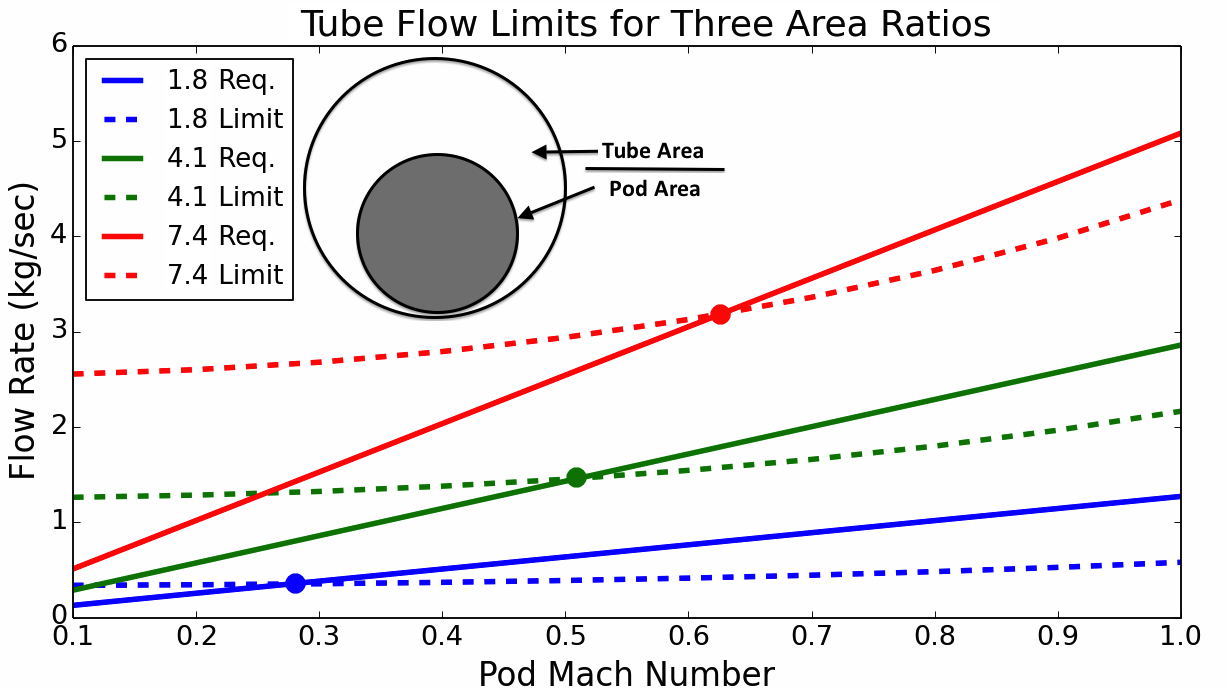
\includegraphics[width=\textwidth]{images/tube_flow_limit3.png}
\caption{Hyperloop speed limits as a function of three different area ratios}
\label{f:flowLIMIT}
\end{figure}

Such low speeds would not allow the Hyperloop concept to significantly reduce travel times between Los Angeles and San Francisco relative
to high speed rail. To reach higher speeds, an inlet and compression system is needed to help draw additional air through the pod.
The vertical distances between the choked flow limit (dashed lines) and the required flow (solid lines) of figure \ref{f:flowLIMIT}
signifies the minimum compressor flow rates necessary to achieve a given speed. 

Additional non-linearity is introduced when considering the limitations of the compression system. Increasing the demands on the compressors
causes the required pod inlet diameter to grow in order to handle the increased flow. Traveling faster results in larger mass flow requirements,
which drives the pod diameter up, subsequently changing the area ratio and further increasing the mass flow requirements.
This compounding relationship between 
speed and tube diameter is shown in figure \ref{f:machRAD}. For each point on this graph, the full system model converges on the minimal
possible tube diameter, given a desired pod Mach number. Figure \ref{f:machRAD} also accounts for compressor performance limitations and
the steady-state operating tube temperature that reaches quiescence above ambient conditions.

\begin{figure}[hbtp]
\centering
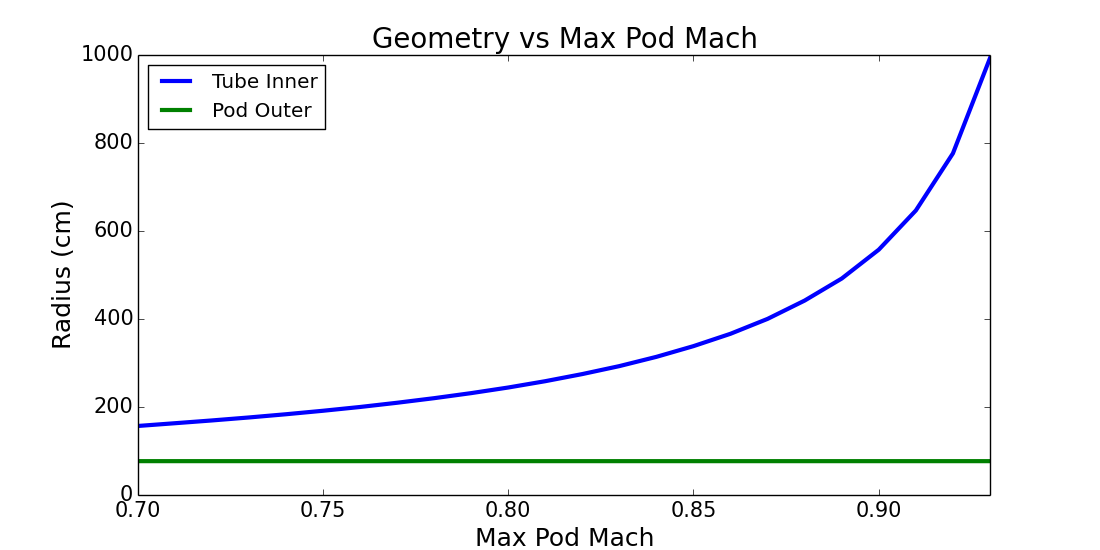
\includegraphics[width=\textwidth]{images/mach_vs_rad2.png}
\caption{Exponential relationship between pod speed and required tube radius}
\label{f:machRAD}
\end{figure}

The exponential relationship between pod max speed and required tube radius explicitly shows the trend depicted by
connecting the dots of figure \ref{f:flowLIMIT}. The absolute tube radius is charted rather than an area ratio for visual simplicity
and as a more of a direct indicator of total system cost. It's worth noting that the pod size is also free to vary at each optimized point
and is plotted on the green line. Somewhat surprisingly, the pod radius remains
nearly constant for every optimization at each targeted speed condition. This can be attributed the extremely sensitive nature of the inlet
size when perturbed in either direction. Decreasing the inlet diameter adversely effects capsule air intake more-so than it helps
bypass air throughput; and increasing the inlet diameter negatively impacts the bypass area at a greater rate than it improves
compressor intake. The inlet size is also somewhat governed by the
necessary bearing flow requirements. Unlike figure \ref{f:flowLIMIT}, this plot accounts for
the capsule compression system and is therefore shifted further right than if the intersection points from figure \ref{f:flowLIMIT}
were translated and directly overlaid. 

The data shows that above Mach .85, the minimum allowable tube size gets very sensitive to pod travel speed. This indicates that speeds
greater than Mach .9 are likely not feasible. Even at a Mach .8, the tube still needs to be approximately 4 meters in diameter, roughly
twice the size considered in the original proposal. With a maximum speed of Mach .8, the travel time is greater than 45 minutes and
additional time would also be necessary to reduce acceleration around banked turns. Although this performance is much less favorable than the performance
described in the original proposal, it still represents an improvement over what can be achieved with a high speed rail.


\subsection{Compression System}

The compression system serves dual purposes. It provide a means of exceeding the nominal Kantrowitz limit
and also supplies pressurized air to support the air bearing system.
Each of these functions requires a minimum airflow to rise to a specific pressure gain,
which combine to define the total airflow requirements for the whole sub-system.
The system is comprised of an inlet, two compressors, two heat exchangers, a nozzle, and multiple ducts leading to air bearings.

\begin{figure}[hbtp]
\centering
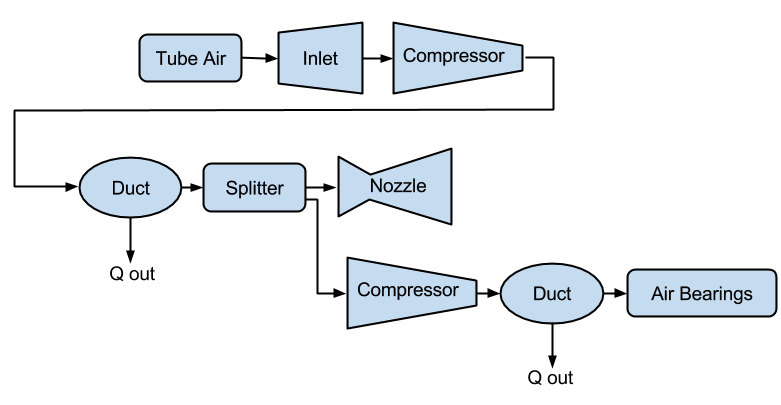
\includegraphics[width=\textwidth]{images/compressor_schematic.png}
\caption{Schematic flow diagram of the modeled compressor system}
\end{figure}

The compression systems is modeled as a one dimensional cycle, representing components as thermodynamic processes that are
subsequently chained together. Each component is responsible for calculating gas properties across its boundaries and appropriately
enforcing conservation equations across the entire system. The subsystem leverages the open-source Cantera package, which is 
responsible for calculating chemical kinetics, thermodynamics, and transport processes. These models predict the instantaneous
power consumption of the compressors, temperature rise, and upstream conditions necessary to supply sufficient airflow to the bearings.
These power requirements are a function of the chosen cycle and are both affected by and contribute to the thermal conditions. 
Combined with the estimated travel time, these requirements impact battery sizing and coolant storage requirements.
The following section provides a brief summary of the assumptions and modeling that went into each sub-system necessary to perform this analysis.

\begin{figure}[H]
\centering
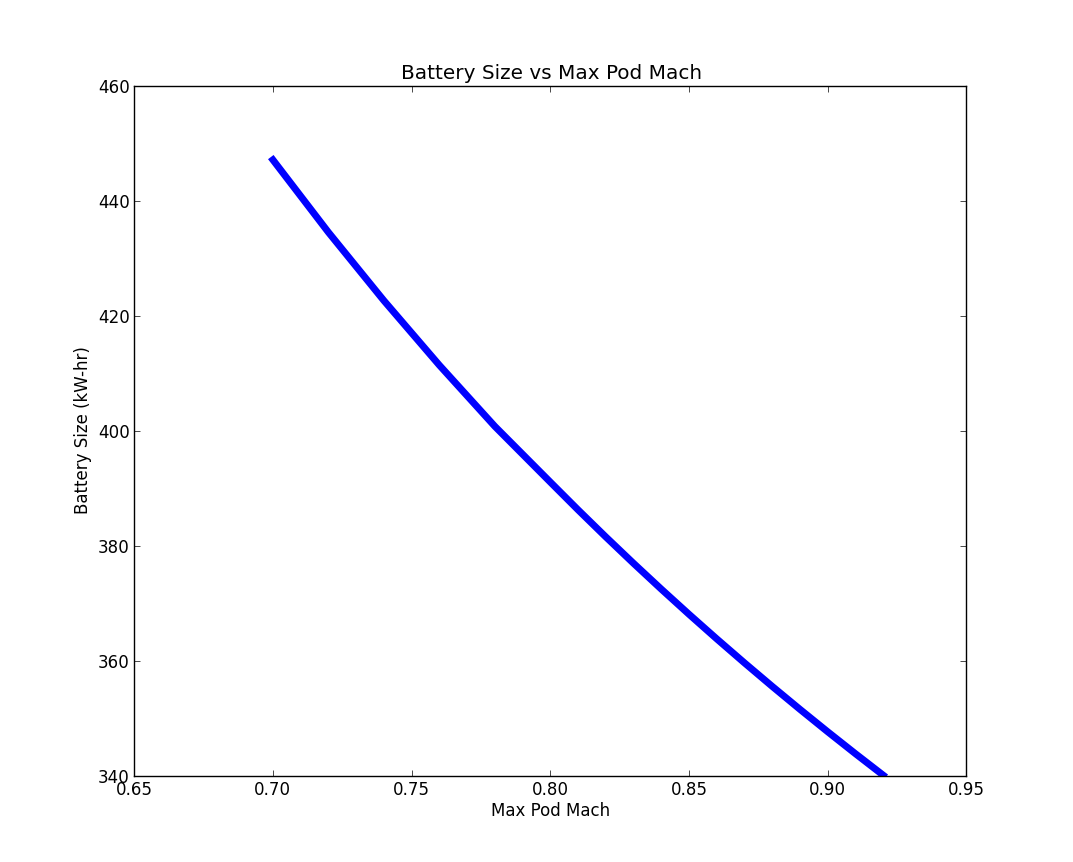
\includegraphics[width=\textwidth]{images/mach_vs_energy.png}
\caption{Battery requirements as a function of pod speed}
\end{figure}

\subsection{Tube Temperature}

As each pod passes through the tube, it adds energy to the air in the form of heat. Considering the frequency of the continuous operating cycle,
this could potentially heat the overall Hyperloop system to excessive temperatures.
To combat this effect, the original proposal recommends a heat exchanger system that would 
be integrated into the compression system. These intercoolers would use water stored in on-board tanks to cool the
air and assist secondary compression. The resulting steam could then be stored in a separate tank and offloaded once the pod reached its destination.
However, initial calculations show that using water for cooling is not an ideal design for two reasons:

1) The flow rate of water needed to remove the heat added by the compressors is very large, and the sheer volume constraints of storing
the resulting steam would outweigh the benefits.

2) The heat addition from each pod compressor cycle is fairly low relative to other heat transfer mechanisms occurring between the Hyperloop
and the external environment. Even without an active on-board cooling solution, the tube temperature would be dominated by other factors.

The following two sections provide additional details about the engineering models used to draw these conclusions.

\subsubsection{Capsule Cooling Requirements}

The limits and requirements of a hypothetical on-board heat exchanger can be estimated with a straightforward energy balance. The
effectiveness of a heat exchanger can be described as the ratio of actual heat transfer over the maximum possible heat transfer.

\begin{equation*}
{Q}_{released}  = effectiveness * {Q}_{max}
\end{equation*}


with $Qmax=\left(T_{hot,in} - T_{cold,in}\right) [ \dot{m} C_{p} ]_{fluid}$ where each fluid has a $\dot{m} C_{p}$ and the fluid with the lowest
product is used to determine the maximum heat transfer. In order to satisfy the energy balance $Q_{released}=Q_{absorbed}$ the following must be true,

\begin{equation*}
\dot{m}_{air} C_{p, air} (T_{out, air} - T_{in, air}) = {Q}_{released} = {Q}_{absorbed}= \dot{m}_{water} C_{p,water} (T_{out, water} - T_{in, water})
\end{equation*}

where the $T_{out}$  of each fluid is unknown. With assumed mass-flow rates and initial temperatures, a valid combination of Tout‘s of
each fluid can be found through solver iteration. Valid effectiveness levels for heat exchangers can be estimated based on the E- NTU
method. The effectiveness for a counter flow heat exchanger with a $\frac{C_{min}}{C_{max}}$ of ~0.25 was chosen with air and water as the working fluids. 
The following conditions satisfied an energy balance with an extremely optimistically assumed effectiveness of 0.9765, and the proposed requirement to fully
cool the air back down to inlet temperatures.

\begin{tabular}{|c|c|c|c|c|c|c|}
\hline 
Fluid & Cp & Tin & Tout & mdot & Q (kJ/s) & Qmax \\ 
\hline 
Air & 1.006 kJ/kh-K & 791 K & 300 K & 0.49 kg/s & -242 & 247.9 \\ 
\hline 
Water & 4.186 kJ/kg-K & 288.15 & 416.6 K  & 0.45 kg/s & 242 & 247.9 \\ 
\hline 
\end{tabular} 


With a 35 minute trip, $0.45 \frac{kg}{s} * 60 \frac{s}{min} * 35min = 945 kg$ of standard temperature/pressure water would need to be carried 
with steam tanks over a hundred meters in length. This doesn't even account for the second stage heat exchanger, making the system nearly infeasible
with water and unpressurized tanks. Various systems involving alternate coolants such as liquid air or pressurized tanks could be explored.

Further discussion of heat exchanger sizing can be found in the heat exchanger section of the appendix.
The calculations explore the possibility of multi-pass heat exchangers
and the logarithmic mean temperature difference (LMTD) of the heat exchanger is considered.

\subsubsection{Equilibrium Tube Temperature}
A high-level assessment of the overall steady-state heat transfer between the 300 mile Hyperloop tube and the ambient atmosphere is
also investigated. The outer diameter of the pipe is chosen as the control surface boundary used in the heat balance. Heat added from the capsule exhaust air and
solar flux were considered the primary drivers for heat absorption into the tube. Conversely, heat released from the tube was modeled by means of
ambient natural convection and radiation out from the stainless-steel surface. The thermal interaction between the rarified internal air and
tube was not modeled.

The heat being added by the pods can be determined from the cycle analysis, or based purely on inlet total temperatures with isentropic
flow relations.

\begin{equation*}
T_{t} = T_{s} * [1 + \frac{\gamma -1}{2} MN^2]
\end{equation*}
\begin{equation*}
P_{t} = P_{s} * (\frac{ T_{t}}{T_{s}})^(\frac{\gamma}{\gamma -1})
\end{equation*}
\begin{equation*}
P_{t,exit} = P_{t,inlet} * PR
\end{equation*}
\begin{equation*}
T_{t,exit} = T_{t,inlet} + \frac{([T_{t,inlet}*PR^{(\frac{\gamma-1}{\gamma})}] - T_{t,inlet})}  {{\eta}_{adiabatic}}
\end{equation*}

Where PR is the compressor pressure ratio, MN is the mach number,  $\gamma$ is the specific heat ratio, and  ${\eta}_{adiabatic}$ is the
adiabatic efficiency.

With the air flow rate known, the heat flow rate per capsule is obtained,

\begin{equation*}
{Q}_{pod}= \dot{m}_{air} C_{p,air} (T_{out, air} - T_{tube})
\end{equation*}
The peak heating rate from the pods scales linearly.
\begin{equation*}
{Q}_{peak}= Q_{pod} (\# ofpods)
\end{equation*}
The solar heat flow per unit area can be approximated, given the solar reflectance index (SRI) of stainless steel, non-normal incidence factor
of the cylinder and solar insulation (SIF).
\begin{equation*}
Solar = (1-SRI) {\theta}_{nni} SIF
\end{equation*}
Multiplying this by the viewing area of the tube (assuming no shade and constant sun)
\begin{equation*}
Q_{solar} = Solar * A_{view} = Solar * L_{tube} * OD_{tube}
\end{equation*}
Tube cooling can be attributed to two general mechanisms, radiation and natural convection. Radiation power per unit area can be
approximated to
\begin{equation*}
\frac{P_{rad}}{A} = \epsilon \sigma (T_{pipe}^4 - T_{ambient}^4)
\end{equation*}
where  $\epsilon$ is the emissivity factor and  $\sigma$ is the Stefan-Boltzmann constant.

Multiplying by the surface area of the tube, the total heating rate can be found,
\begin{equation*}
P_{rad} =  \frac{P_{rad}}{A} * \pi L_{tube} OD_{tube}
\end{equation*}

Assuming the worst case scenario of no cross wind, convection is primarily driven by temperature gradients. The non-dimensional relation
between buoyancy and viscosity driven flows is parameterized using the following empirical constants. \cite{Berton} \cite{Incropera}

if 150 K $<  T_{amb} <$ 400 K:

\begin{equation*}
\frac{g \beta T} {\upsilon^2} = (m^{-3}K^{-1}) = 4.178\times10^{19} \times T_{amb}^{-4.639}
\end{equation*}

\begin{equation*}
Pr = 1.23 T_{amb}^{-0.09685}
\end{equation*}

if 400 K $<  T_{amb}  <$ 2100 K:


\begin{equation*}
\frac{g \beta T} {\upsilon^2}  = (m^{-3}K^{-1}) = 4.985\times10^{18} \times T_{amb}^{-4.284}
\end{equation*}
\begin{equation*}
Pr = 0.59 T_{amb}^{0.0239}
\end{equation*}
The Grashof Number can then be approximated,


\begin{equation*}
Gr = \frac{g \beta T} {\upsilon^2}  (T_{tube}-T_{amb}) {OD}_{tube}^3
\end{equation*}
The non-dimensional Rayleigh number can then be calculated to estimate buoyancy effects, leading to the Nusselt number.


\begin{equation*}
Ra = Gr * Pr
\end{equation*}
\begin{equation*}
Nu = \Bigg(0.6 + \frac{0.387Ra^{\frac{1}{6}}}{[1+(\frac{0.559}{Pr})^{\frac{9}{16}}]^{\frac{8}{27}}}\Bigg)^2
\end{equation*}

From this point the total heat transfer from natural convection can be obtained,

\begin{equation*}
Q_{nat. conv} = hA \Delta T = \frac{k*Nu}{ {OD}_{tube}} \pi {L}_{tube} {OD}_{tube} (T_{tube}-T_{amb})
\end{equation*}

The steady state tube temperature can be found by varying the tube temperature until the rate of heat being released from the tube
matches the rate of heat being absorbed by the tube. Assuming numerous state variables provided in the source code, a steady state temperature of 120 F
was reached. These result suggests that there is no need for on-board cooling, however many baseline assumptions have yet to be validated or even defined.

\section{Full Model Integration}
The model is broken down into 5 major assemblies as described below. 

\begin{enumerate}
  \item Compression System (\texttt{compress}): Performance and power consumption of the compressors
  \item Mission Analysis (\texttt{mission}): Estimate of travel time
  \item Pod Geometry (\texttt{pod}): Physical dimensions of the capsule and calculations that depend on them
  \item Tube Flow Limitations (\texttt{flow\_limit}): Pod speed limitations based on choked flow restrictions between the pod and the tube
  \item Tube Wall Temperature (\texttt{tube\_wall\_temp}): Equilibrium temperature of the tube wall
\end{enumerate}

The connectivity between the assemblies is visually represented using XDSM charts below. Each green box represents a system that takes a
set of inputs and operates on them to produce a set of outputs. The connection of one system's outputs to another system's inputs is
visualized as a grey line. The cascading parallelograms indicate intersections, implying that an output is connected to multiple inputs. 


\begin{figure}[hbtp]
\centering
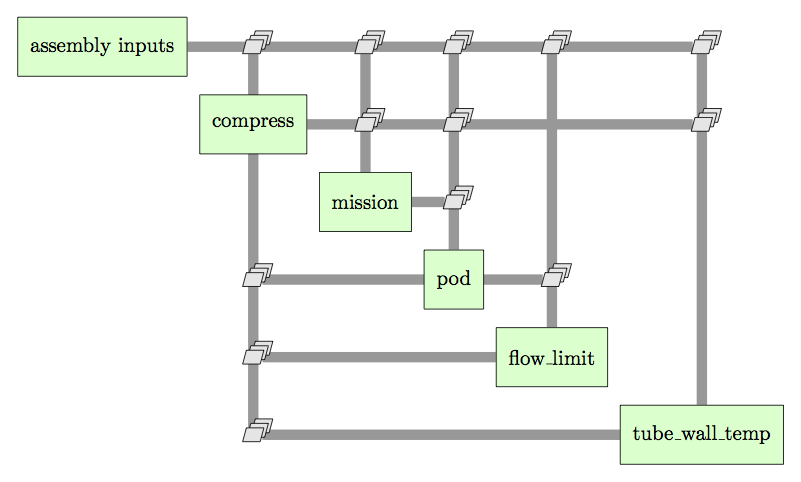
\includegraphics[width=\textwidth]{images/hyperloop_assembly_xdsm.png}
\caption{Hyperloop Top Level Assembly XDSM}
\label{f:hyperloopXDSM}
\end{figure}

The compression system and pod geometry systems in figure \ref{f:hyperloopXDSM} are further expanded into sub-assemblies as shown in figure \ref{f:podXDSM} and \ref{f:compressorXDSM}.

\begin{figure}[hbtp]
\centering
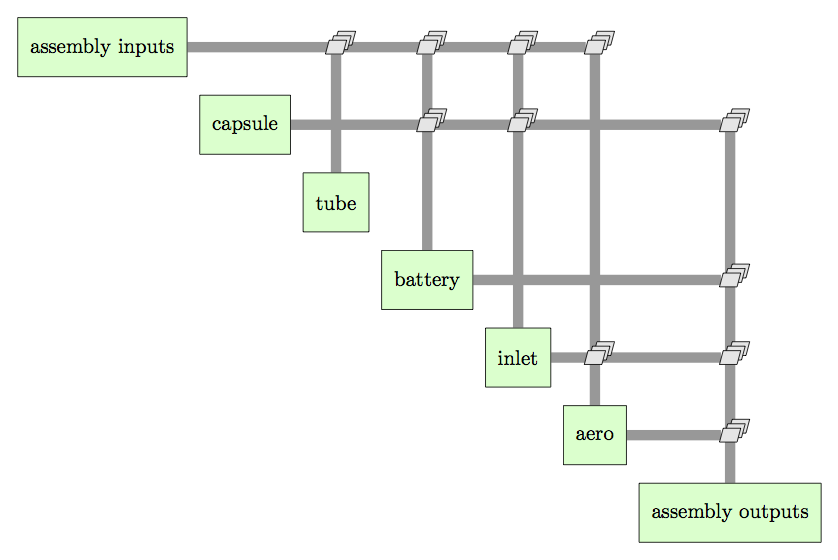
\includegraphics[width=\textwidth]{images/pod_assembly_xdsm.png}
\caption{Expanded \texttt{pod} assembly XDSM}
\label{f:podXDSM}
\end{figure}

\begin{figure}[hbtp]
\centering
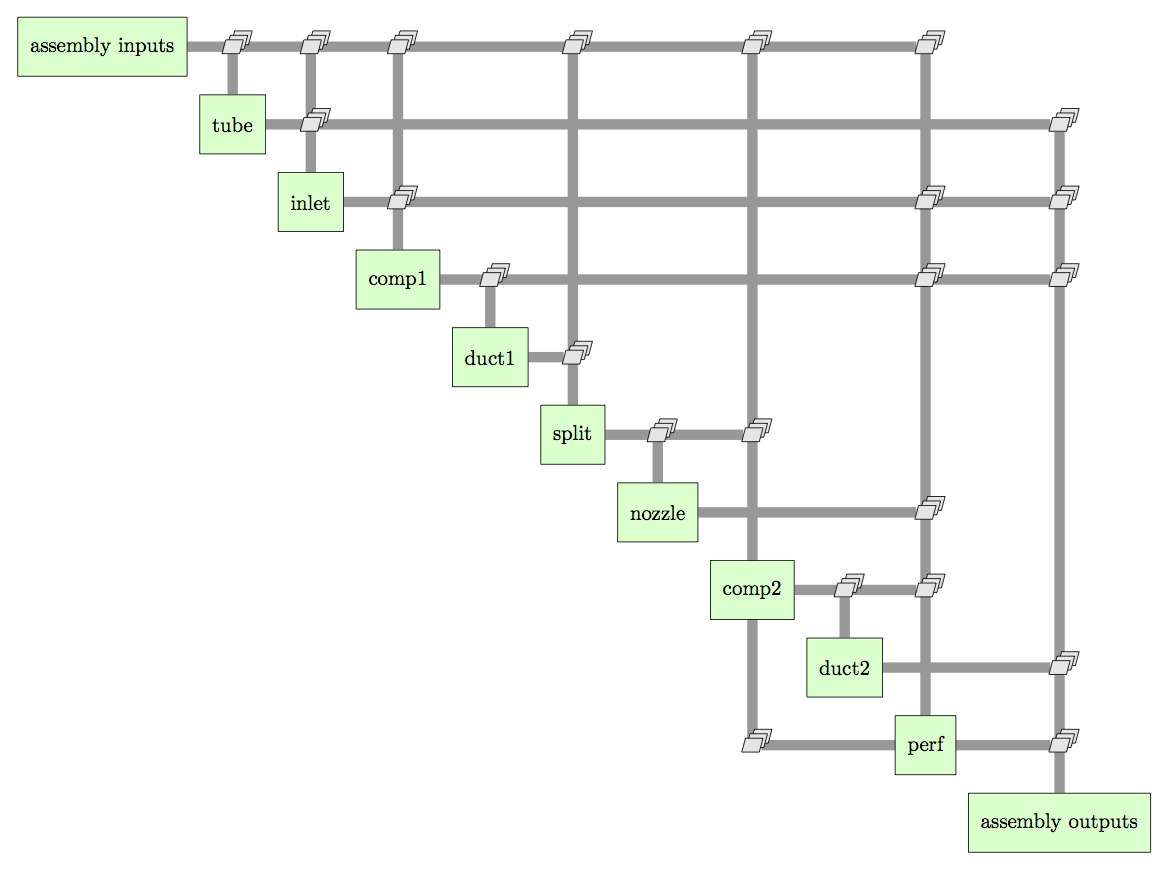
\includegraphics[width=\textwidth]{images/compress_assembly_xdsm.png}
\caption{Expanded \texttt{compress} assembly XDSM}
\label{f:compressorXDSM}
\end{figure}

\subsection{Design Variables}
The system design is defined at the top-most level with the following design variables. These variables can be actively varied
 by the optimizer to achieve user defined objectives:

\begin{adjustwidth}{-2cm}{-2cm}
\begin{tabular}{|c|c|c|c|c|c|}
\hline 
Variable & Description & Units & Baseline Val. & Min & Max \\ 
\hline 
\texttt{Mach\_bypass} & Mach number of the air traveling around the pod & - & 0.95 & 0.5 & 0.98 \\ 
\hline 
\texttt{Mach\_pod\_max} & Maximum travel Mach number of the pod & - & 0.9 & 0.5 & 0.98 \\ 
\hline 
\texttt{Mach\_c1\_in} & Mach number of the air at the back of the inlet & - & 0.6 & 0.5 & 0.8 \\ 
\hline 
\texttt{Ps\_tube} & Static pressure of the air in the tube & Pa & 99 & 99 & 500 \\ 
\hline 
\texttt{c1\_PR\_des} & First compressor pressure ratio & - & 12.47 & 10 & 25 \\ 
\hline 
\end{tabular} 
\end{adjustwidth}

\subsection{Model Parameters}
These variables are free for the user to set, but are not intended for the optimizer. Rather, they are general traits of the system.

\begin{adjustwidth}{-3cm}{-3cm}
\begin{tabular}{|c|c|c|c|c|c|}
\hline 
Variable & Description & Units & Baseline Val & Min. & Max. \\ 
\hline 
pwr\_marg & Safety factor applied to the power requirement for the pod & - & 0.3 & 0 & 2 \\ 
\hline 
solar\_heating\_factor & Fraction of solar radiation to consider in tube temperature & - & 0.7 & 0 & 1 \\ 
\hline 
tube\_length & Length of the tube & m & 563270 & - & - \\ 
\hline 
n\_rows & Number of rows of seats in the passenger capsule & - & 14 & - & - \\ 
\hline 
length\_row & Length allotted to each row of seats & cm & 150 & 120 & 200 \\ 
\hline 
coef\_drag & Drag Coefficient for the pod & - & 2 & 0.6 & 2.5 \\ 
\hline 
hub\_to\_tip & Ratio of hub radius to tip radius for the first compressor & - & 0.4 & 0.2 & 0.6 \\ 
\hline 
\end{tabular} 
\end{adjustwidth}

\subsection{Constraints and State Variables}

The Hyperloop concept presents a multidisciplinary design problem and encapsulating complexity into systems makes the relationship
between variables easier to understand.  Any connection originating from the left side of a component in an XDSM diagram represents a
cyclic connection. The cyclic connections in figure \ref{f:hyperloopXDSM}  and \ref{f:compressorXDSM} represent the coupling relationships
between the sub-systems. These couplings enforce a set of equality constraints that must be satisfied for any physically valid Hyperloop design. 

\begin{equation} \label{eq:flow}
	0.01*(\texttt{compress.W\_in} - \texttt{flow\_limit.W\_excess}) = 0
\end{equation}
\begin{equation}
	\texttt{compress.Ps\_bearing\_residual} = 0
\end{equation}
\begin{equation}
	\texttt{tube\_wall\_temp.ss\_temp\_residual} = 0
\end{equation}
\begin{equation} \label{eq:area}
	0.01*(\texttt{pod.area\_compressor\_bypass} - \texttt{compress.area\_c1\_out}) = 0
\end{equation}

For constraints \ref{eq:flow} and \ref{eq:area}, a multiplier has been applied to the constraint to scale it for improved numerical
convergence.

The optimizer varies  the following state variables to to satisfy the constraints. 

\begin{enumerate}
\item \texttt{compress.W\_in}
\item \texttt{compress.c2\_PR\_des}
\item (\texttt{compress.Ts\_tube}, \texttt{flow\_limit.Ts\_tube}, \texttt{tube\_wall\_temp.temp\_boundary}) \label{Temp}
\item (\texttt{flow\_limit.radius\_tube}, \texttt{pod.radius\_tube\_inner}) \label{Radius}
\end{enumerate}

State variables \ref{Temp} and \ref{Radius} are given as a list of variables signifying that they are linked variables with equivalent values. They are
treated as a single variable for the purposes of converging the model, but remain as distinct variables within each subsystem.

\subsection{Outputs}
There are a number of output values that are of interest

\begin{description}
  \item[Overall pod radius] \hfill \\
  \texttt{pod.radius\_inlet\_outer}
  \item[Total mass flow through the compression system] \hfill \\
  \texttt{compress.W\_in}
  \item[Total power required to drive the compression system] \hfill \\
  \texttt{compress.pwr\_req}
  \item[Total energy needed to power the compression system for one trip] \hfill \\
  \texttt{mission.energy}
  \item[Travel time for one trip] \hfill \\
  \texttt{mission.time}
  \item[Maximum speed] \hfill \\
  \texttt{compress.speed\_max}
  \item[Equilibrium tube temperature] \hfill \\
  \texttt{tube\_wall\_temp.temp}
\end{description}

Note: For a more complete design process, the values of the design variables would be optimized to minimize a combination of total power
consumption and travel time. However, the model does not currently calculate some key values needed to get a useful answer. In particular,
the linear accelerator and vacuum pump power needs to be modeled before a design optimization can be attempted.
It should be noted that you can select designs that are not realistic, particularly with respect to \texttt{pod.radius\_inlet\_outer}. There is
a strong relationship between \texttt{Mach\_pod\_max} and the \texttt{pod.radius\_inlet\_outer}. If you select a high 
\texttt{Mach\_pod\_max} (Above .8), you may find that the radius has shrunk below what is physically feasible without significant design
changes.


\section{Conclusions}
For the most part, the ideas and numbers given in the original Hyperloop proposal hold up using this analysis. However, the data shows that
there are two major changes to the design that need to be considered.

The tube cross section will need to be significantly larger than the original proposal. In the original proposal, the tube was sized with a diameter 2.23
meters. However, it appears that it will need to have a diameter closer to 4 meters to reach speeds maximum speeds of Mach 0.8.
On-board water based inter-coolers also seem impractical due to both volume and weight constraints. This may prove to be a non-issue since
temperature rise due to compression is significant less than originally estimated and only leads to a modest rise in steady-state tube
temperature. Assuming the tube was left uncovered, the heat rate from solar radiation would be an order of magnitude larger than the heat
rate added from pod compression systems. Further assuming a 90 degF day, radiation and convection out of the tube would lead to a
manageable steady state tube wall temperature of 120 degF.

%\begin{thebibliography}{WoodTP}
%\bibitem[WoodTP]{woodTP} Wood, W.A., ``Multidimensional Upwind
 % Fluctuation Splitting Scheme with Mesh Adaption for Hypersonic Viscous
 % Flow,'' NASA/TP 2002-211640, Apr.~2002.
%\end{thebibliography}
%{\em Note that this entry is not necessarily in the correct NASA
%  format. Consult Technical Editing for correct reference format.}
\end{document}
